% Этот шаблон документа разработан в 2017 году
% Владимиром Коротковым (kvamob@mail.ru) 
%  

\documentclass[a4paper,12pt]{article} % добавить leqno в [] для нумерации слева

%% Глобальные Параметры страницы
\usepackage[left=3cm,right=2cm,top=1cm,bottom=2cm,bindingoffset=0cm]{geometry}

%\usepackage{fp} 						% Вычисления с плавающей точкой
%\usepackage{siunitx}					% При использовании пакета fp все числа должны иметь decimal delimiter точку
%\sisetup{output-decimal-marker={,}}	% Числа выводятся с запятой в качестве разделителя разрядов: \num{3.2} выводит 3,2 

%%% Работа с русским языком
\usepackage{cmap}					% поиск в PDF
\usepackage{mathtext} 				% русские буквы в формулах
\usepackage[T2A]{fontenc}			% кодировка
\usepackage[utf8]{inputenc}			% кодировка исходного текста
\usepackage[english,russian]{babel}	% локализация и переносы

%%% 
%\usepackage{rotating}				% Поворот текста

%%% Дополнительная работа с математикой
\usepackage{amsmath,amsfonts,amssymb,amsthm,mathtools} % AMS
\usepackage{icomma} % "Умная" запятая: $0,2$ --- число, $0, 2$ --- перечисление

%% Номера формул
%\mathtoolsset{showonlyrefs=true} % Показывать номера только у тех формул, на которые есть \eqref{} в  тексте.

%% Шрифты
\usepackage{euscript}	 % Шрифт Евклид
\usepackage{mathrsfs} % Красивый матшрифт


%% Перенос знаков в формулах (по Львовскому)
% \newcommand*{\hm}[1]{#1\nobreak\discretionary{}
%	{\hbox{$\mathsurround=0pt #1$}}{}}

%%% Работа с картинками
\usepackage{graphicx}  % Для вставки рисунков
%\usepackage[export]{adjustbox}
\graphicspath{{images/}{images2/}}  % папки с картинками
\setlength\fboxsep{3pt} % Отступ рамки \fbox{} от рисунка
\setlength\fboxrule{0.2pt} % Толщина линий рамки \fbox{}
\usepackage{wrapfig} % Обтекание рисунков и таблиц текстом


%%% Работа с таблицами
\usepackage{array,tabularx,tabulary,booktabs} % Дополнительная работа с таблицами
\usepackage{longtable}  % Длинные таблицы
\usepackage{multirow} % Слияние строк в таблице

%%% Подписи к рисункам и таблицам в русской типографской традиции
\usepackage{caption} 
\DeclareCaptionFormat{GOSTtable}{#2#1\\#3}
\DeclareCaptionLabelSeparator{fill}{\hfill}
\DeclareCaptionLabelSeparator{dot}{. }
\DeclareCaptionLabelFormat{fullparents}{\bothIfFirst{#1}{~}#2}
\captionsetup[table]{
	format=GOSTtable,
	font={footnotesize},
	labelformat=fullparents,
	labelsep=fill,
	labelfont=rm,
%	labelfont=it,
	textfont=bf,
	justification=centering,
	singlelinecheck=false
}
\captionsetup{font=small}
\captionsetup[figure]{
	labelsep=dot, 
%	textfont=it
}
% А можно и так
%\captionsetup{labelsep=period}


%%% Модификация команд, задающих разделы
% Не подавлять отступы у первого абзаца

\makeatletter   % Команда \makeatletter делает символ @ буквой, команда \makeatother возвращает всё на свои места.
% Разрешим отступ у первого абзаца
\renewcommand\section{\@startsection {section}{1}{\parindent}%
	{3.5ex \@plus 1ex \@minus .2ex}{2.3ex \@plus.2ex}%
	{\normalfont\hyphenpenalty=10000\Large\bfseries}}

\renewcommand\subsection{\@startsection {subsection}{1}{\parindent}%
	{3.5ex \@plus 1ex \@minus .2ex}{2.3ex \@plus.2ex}%
	{\normalfont\hyphenpenalty=10000\large\bfseries}}

\makeatother

% После номеров разделов \section ставить точки
\usepackage{secdot}			
% И после \subsection тоже ставить точки
\sectiondot{subsection}		

\usepackage{setspace} % Интерлиньяж
%\onehalfspacing % Интерлиньяж 1.5
%\doublespacing % Интерлиньяж 2
%\singlespacing % Интерлиньяж 1

\usepackage{lastpage} % Узнать, сколько всего страниц в документе.

\usepackage{soulutf8} % Модификаторы начертания

%\usepackage{hyperref}
%\usepackage[usenames,dvipsnames,svgnames,table,rgb]{xcolor}
%\hypersetup{				% Гиперссылки
%	unicode=true,           % русские буквы в раздела PDF
%	pdftitle={Заголовок},   % Заголовок
%	pdfauthor={Автор},      % Автор
%	pdfsubject={Тема},      % Тема
%	pdfcreator={Создатель}, % Создатель
%	pdfproducer={Производитель}, % Производитель
%	pdfkeywords={keyword1} {key2} {key3}, % Ключевые слова
%	colorlinks=true,       	% false: ссылки в рамках; true: цветные ссылки
%	linkcolor=red,          % внутренние ссылки
%	citecolor=green,        % на библиографию
%	filecolor=magenta,      % на файлы
%	urlcolor=cyan           % на URL
%}

\usepackage{multicol} % Несколько колонок

\usepackage{fancyhdr} % Колонтитулы
%\pagestyle{fancy}
%\renewcommand{\headrulewidth}{0mm}  % Толщина линейки, отчеркивающей верхний колонтитул
%\lfoot{Нижний левый}
%\rfoot{Нижний правый}
%\rhead{Верхний правый}
%\chead{Верхний в центре}
%\lhead{Верхний левый}
% \cfoot{Нижний в центре} % По умолчанию здесь номер страницы


%%%%%%%%%%%%%%%%%%%%%%%%%%%%%%%%%%%%%%%%%%%%%%%%%%%%%%%%%%%%%%%%%%%%%%%%%%%%%%%%%%%%%%%%%%%%%%%%%%%%%%%%%
%%% PAYLOAD
%%%%%%%%%%%%%%%%%%%%%%%%%%%%%%%%%%%%%%%%%%%%%%%%%%%%%%%%%%%%%%%%%%%%%%%%%%%%%%%%%%%%%%%%%%%%%%%%%%%%%%%%%

%%% Заголовок
\author{ООО <<Гидросфера>>}\label{company}
\title{ОТЧЕТ ПО РЕЗУЛЬТАТАМ РАСЧЕТА ДРЕНАЖНОЙ СИСТЕМЫ}
\date{\today}
%%%======================================================================================================
\newcommand{\txtExecutor}{ООО <<Гидросфера>>}	% Исполнитель
\newcommand{\txtYear}{2017}						% Год
\newcommand{\txtAddress}{Свердловская область, р.п. Верхнее Дуброво, ул. Рябиновая, 17}			% Адрес
\newcommand{\txtCadaster}{66:66:0101003:545,450} 		% Кадастровый номер

%% ГИДРОГЕОЛОГИЧЕСКИЕ УСЛОВИЯ - Раскомментарить одно из:
%\newcommand{\hydrogeology}{\textbf{Трещинные воды}. Уральская сложная гидрогеологическая складчатая область располагается в пределах орографически выраженного одноименного горно - складчатого сооружения. Основными коллекторами подземных вод являются трещиноватые породы коренного субстрата. Мощность зоны региональной трещиноватости составляет в среднем 30 – 100 м. Минимальные значения (20 – 30 м) присущи корам выветривания интрузивных пород; максимальные (60 – 100 м) – карбонатным породам; средние (40 – 60 м) – эффузивно-осадочным и метаморфическим комплексам. Помимо трещин выветривания широко развиты локальные линейные трещинные зоны высокой проницаемости и водоотдачи, связанные с проявлениями дизъюнктивной тектоники и контактами разнородных пород. Подземные воды региональной трещиноватости обычно гидравлически взаимосвязаны, имеют безнапорный характер и образуют небольшие бассейны с интенсивным
водообменном. В вертикальном разрезе фильтрационные свойства пород зоны выветривания неоднородны. По характеру их изменения зона разделяется на три части. В верхней (10 – 20 м), где широко представлены глины или суглинки элювиальной коры выветривания, водопроницаемые свойства очень низки; особенно широко коры распространены на площади Зауральского пенеплена. Средняя часть эрозионной зоны отличается наибольшей активностью, сильной степенью трещиноватости и высокой пористостью (от 1 до 7 \%). В нижней части размеры трещин весьма незначительны, и водоотдача пород практически отсутствует.

\textit{Водоносная зона трещиноватости позднепалеозойских интрузивных кислых и средних пород} ($\gamma PZ_3$) связана с массивами гранитов, гранодиоритов, плагиогранитов, диоритов. Региональная зона выветривания на этих массивах не превышает 15 – 20 м, зеркало подземных вод в сглаженной форме повторяет современный рельеф. Водоносность зоны крайне неравномерна: в центральных частях массивы практически безводны; по периферии (в приконтактовых частях с другими породами) водоносность возрастает до 0,2 – 0,3 л/с. В частности в тектонических и приконтактовых зонах позднепалеозойского Верхисетского гранитного массива отдельные скважины имели дебит до 7,0 л/с при удельном дебите 2,4 л/с, в центре массива оставаясь безводными. Минерализация вод – в пределах 0,08–0,5 г/дм\textsuperscript{3}; по составу преобладают гидрокарбонатные  кальциево-магниевые.

Гранодиориты и плагиограниты становятся более водоносными за счет секущих позднепалеозойских даек и жил «обновленных», к тому же тектоническими движениями создавшими условия для локализации трещинно-жильных вод в зоне выветривания. В окраинных частях Сысертского массива гранодиоритов и плагиогранитов дебиты скважин изменяются от 1,5 до 10,0 л/с при удельных дебитах 0,1 – 8,0 л/с. В центральной части (где нет жильных тел) в маломощной зоне выветривания дебиты скважин не превышают 0,3 – 0,5 л/с при удельных дебитах 0,001–0,01 л/с. Ближе к периферии фиксируютя мелкие источники с расходом 0,1 – 0,2 л/с. По минерализации и химическому составу воды аналогичны развитым в гранитных массивах. 

В целом питание подземных вод Большеуральского бассейна сезонное, за счет инфильтрации атмосферных осадков в теплый период года. Зеркало его вод в сглаженной форме повторяет основные элементы рельефа. На склонах и уплощенных водоразделах уровни воды залегают на глубинах 5 – 20 м, на хребтах и локальных возвышенностях – до 30 – 50 м. Сравнительно глубокая расчлененность дневной поверхности, особенно в районах приподнятых горных массивов, обеспечивает хорошие условия дренирования водоносных зон речной сетью. Разгрузка вод идет преимущественно вдоль долин рек, а также может быть приурочена к локальным трещинным зонам. Дебиты родников, в зависимости от величины водосборной площади, варьируют от долей до многих десятков литров в секунду.

Эксплуатационные ресурсы Большеуральского бассейна связываются преимущественно с крупными карбонатными массивами среднего и верхнего палеозоя и тектонически активными зонами разломов, на которых возможна организация водозаборов с дебитом 100 – 1000 л/с. На остальных водоносных зонах трещиноватости возможен каптаж подземных вод по отдельным кустам скважин с дебитами от 10 до 30 л/с. Ресурсы порово-пластовых вод Иртыш-Обского бассейна связаны преимущественно с опоковым горизонтом палеоцена, мощность обводненной толщи которого 3 – 4 м на западе и до 50 м на востоке. На придолинных участках некоторые водозаборы из него имеют производительность до 50–100 л/с.

Несмотря на значительное количество водоносных горизонтов на изученной площади, наиболее промышленные и обжитые районы Урала испытывают недостаток в водообеспеченности из-за неравномерного распределения ресурсов, а также в связи с невозможностью создания крупных водозаборов с высокой производительностью на локальных участках водоносных зон.
}			% Гранитные интрузии
\newcommand{\hydrogeology}{\textbf{Трещинные воды}. Уральская сложная гидрогеологическая складчатая область располагается в пределах орографически выраженного одноименного горно - складчатого сооружения. Основными коллекторами подземных вод являются трещиноватые породы коренного субстрата. Мощность зоны региональной трещиноватости составляет в среднем 30  --  100~м. Минимальные значения (20  --  30~м) присущи корам выветривания интрузивных пород; максимальные (60  --  100~м)  --  карбонатным породам; средние (40  --  60~м)  ---  эффузивно-осадочным и метаморфическим комплексам. Помимо трещин выветривания широко развиты локальные линейные трещинные зоны высокой проницаемости и водоотдачи, связанные с проявлениями дизъюнктивной тектоники и контактами разнородных пород. Подземные воды региональной трещиноватости обычно гидравлически взаимосвязаны, имеют безнапорный характер и образуют небольшие бассейны с интенсивным
водообменном. В вертикальном разрезе фильтрационные свойства пород зоны выветривания неоднородны. По характеру их изменения зона разделяется на три части. В верхней (10  --  20~м), где широко представлены глины или суглинки элювиальной коры выветривания, водопроницаемые свойства очень низки; особенно широко коры распространены на площади Зауральского пенеплена. Средняя часть эрозионной зоны отличается наибольшей активностью, сильной степенью трещиноватости и высокой пористостью (от 1 до 7~\%). В нижней части размеры трещин весьма незначительны, и водоотдача пород практически отсутствует.

\textit{Водоносная зона трещиноватости средне-верхнепалеозойских карбонатных образований} ($сPZ_{2–3}$) является одной из наиболее водообильных. Она развита преимущественно в пределах синклинальных, реже антиклинальных структурных форм в виде отдельных разобщенных либо взаимосвязанных между собой водоносных горизонтов меридионального и субмеридионального простирания. Наиболее изученные Невьянская, Алапаевская,
Каменская зоны имеют площади до 200 км\textsuperscript{2}. Водовмещающими породами являются известняки с пачками и прослоями глинистых сланцев, аргиллитов, песчаников и туффитов. Трещиновато-карстовая зона имеет мощность 50  --  80~м, достигая в зонах тектонических нарушений 200  --  250~м. С поверхности карбонатные породы осложнены проявлениями карста (в виде воронок); в пределах мезозойских депрессий карст перекрыт кайнозойскимиотложениями, мощность до 20  --  30~м.

Карстовым процессам подвержены все карбонатные «массивы», но степень их проявления неравномерна. На Алапаевском «массиве» скважинами выявлены погребенные щелевидные депрессии длиной до 900  --  2000~м
при ширине 400  --  500~м и глубиной от 70 до 140~м в осевой части.

Характерной особенностью древних карстовых депрессий является высокая трещиноватость бортовых частей и слабая водонасыщенность днищ. Погребенные карстово - трещинные воды в депрессиях обладают напором, соответствующим мощности экранирующего покрова. Питание подземных вод осуществляется за счет инфильтрации атмосферных осадков и разгрузки сопряженных вод из других горизонтов. Циркуляция происходит по сложному лабиринту карстовых пустот и трещин, коэффициент фильтрации в которых варьирует от 2  --  5 до 30~м/сут. Максимальная водообильность приурочена к придолинным участкам пересечения с линейными водоносными зонами. Дебиты родников в них достигают 10  --  25~л/с; в стороне от речных долин вне водоносных зон дебиты не превышают 3  --  5~л/с. Химический состав и минерализация трещинно-карстовых вод изменяются в меридиональном направлении: до широты г. Алапаевск преобладают гидрокарбонатные кальциевые, реже кальциево-магниевые воды с минерализацией от 0,1 до 0,4 г/дм\textsuperscript{3}; южнее распространены гидрокарбонатные кальциево-магниевые, реже кальциевые воды с минерализацией от 0,2 до 0,6 -- 0,8 г/дм\textsuperscript{3}.

В целом питание подземных вод Большеуральского бассейна сезонное, за счет инфильтрации атмосферных осадков в теплый период года. Зеркало его вод в сглаженной форме повторяет основные элементы рельефа. На склонах и уплощенных водоразделах уровни воды залегают на глубинах 5  --  20~м, на хребтах и локальных возвышенностях  ---  до 30  --  50~м. Сравнительно глубокая расчлененность дневной поверхности, особенно в районах приподнятых горных массивов, обеспечивает хорошие условия дренирования водоносных зон речной сетью. Разгрузка вод идет преимущественно вдоль долин рек, а также может быть приурочена к локальным трещинным зонам. Дебиты родников, в зависимости от величины водосборной площади, варьируют от долей до многих десятков литров в секунду.

Эксплуатационные ресурсы Большеуральского бассейна связываются преимущественно с крупными карбонатными массивами среднего и верхнего палеозоя и тектонически активными зонами разломов, на которых возможна организация водозаборов с дебитом 100  --  1000~л/с. На остальных водоносных зонах трещиноватости возможен каптаж подземных вод по отдельным кустам скважин с дебитами от 10 до 30~л/с. Ресурсы порово-пластовых вод Иртыш-Обского бассейна связаны преимущественно с опоковым горизонтом палеоцена, мощность обводненной толщи которого 3  --  4~м на западе и до 50~м на востоке. На придолинных участках некоторые водозаборы из него имеют производительность до 50 -- 100~л/с.

Несмотря на значительное количество водоносных горизонтов на изученной площади, наиболее промышленные и обжитые районы Урала испытывают недостаток в водообеспеченности из-за неравномерного распределения ресурсов, а также в связи с невозможностью создания крупных водозаборов с высокой производительностью на локальных участках водоносных зон.
}		% Карбонтаные образования 
%\newcommand{\hydrogeology}{\textbf{Трещинные воды}. Уральская сложная гидрогеологическая складчатая область располагается в пределах орографически выраженного одноименного горно - складчатого сооружения. Основными коллекторами подземных вод являются трещиноватые породы коренного субстрата. Мощность зоны региональной трещиноватости составляет в среднем 30  --  100~м. Минимальные значения (20  --  30~м) присущи корам выветривания интрузивных пород; максимальные (60  --  100~м)  ---  карбонатным породам; средние (40  --  60~м)  ---  эффузивно-осадочным и метаморфическим комплексам. Помимо трещин выветривания широко развиты локальные линейные трещинные зоны высокой проницаемости и водоотдачи, связанные с проявлениями дизъюнктивной тектоники и контактами разнородных пород. Подземные воды региональной трещиноватости обычно гидравлически взаимосвязаны, имеют безнапорный характер и образуют небольшие бассейны с интенсивным водообменном. В вертикальном разрезе фильтрационные свойства пород зоны выветривания неоднородны. По характеру их изменения зона разделяется на три части. В верхней (10  --  20~м), где широко представлены глины или суглинки элювиальной коры выветривания, водопроницаемые свойства очень низки; особенно широко коры распространены на площади Зауральского пенеплена. Средняя часть эрозионной зоны отличается наибольшей активностью, сильной степенью трещиноватости и высокой пористостью (от 1 до 7 \%). В нижней части размеры трещин весьма незначительны, и водоотдача пород практически отсутствует.

\textit{Водоносная зона трещиноватости нижнепалеозойских ультраосновных пород} ($\Sigma PZ_1$)
связана с перидотитами, дунитами и полнопроявленными серпентинитами, образующими в рельефе значительные возвышенности субмеридионального простирания с ограниченными бассейнами питания трещинных грунтовых вод. Породы весьма устойчивы к процессам выветривания; мощности трещиноватой зоны не превышают 10  --  15~м. В центральных частях массивы практически безводны, а в окраинных расход родников варьирует от 0,01 до 0,2  --  0,3~л/с. Дебиты скважин, вскрывших выветрелые трещиноватые серпентиниты, не превышают 1,5 -- 2,5~л/с.

Наибольшая обводненность приурочена к периферийным разломам, обновленным неотектоникой. В частности, по отдельным данным, восточная часть Колинского серпентинитового массива (в районе г. Серов) «срезана» в плане и опущена на 200~м региональным ступенчатым сбросом, прослеживаемым на 150 км. Вдоль этого нарушения ультрамафиты трещиноваты и аккумулируют подземный сток грунтовых вод зоны выветривания. Дебиты
скважин в этой зоне изменяются от 5 до 30~л/с при удельных дебитах 0,5  --  6,5~л/с. По периферии других массивов водоносность нередко связана с жилами и дайками кислого и основного составов, имеющими более молодой возраст. Грунтово-трещинные и трещинно-жильные воды имеют минерализацию 0,1 -- 0,5 г/дм\textsuperscript{3}, и лишь на отдельных массивах встречаются ультрапресные воды. По химическому составу они гидрокарбонатные магниевые или гидрокарбонатные магниево-кальциевые. Высокие показатели магния обусловлены большим содержанием его окиси в коренных породах.

Водоносные горизонты зон высокой проницаемости и водоотдачи приурочены к омоложенным в новейшее время дизъюнктивам. Детально одна из таких тектонических зон была изучена А. В. Скалиным в Екатеринбурге
при инженерно-геологических изысканиях под высотные здания в центре города. Она приурочена к контакту габбрового массива с вулканогенной толщей и имеет ширину до 60~м. Коэффициент фильтрации здесь составляет 10  --  20~м/сут (трещиноватое габбро  --  до 1~м/сут). При опытных откачках дебит скважин в трещиноватых габбро не превышает 1,4 дм\textsuperscript{3}/с, в тектонической зоне  ---  3,5 дм\textsuperscript{3}/с. Суммарный дебит последней по кустовой откачке трех скважин составил 950~м\textsuperscript{3}/сут.

В целом питание подземных вод Большеуральского бассейна сезонное, за счет инфильтрации атмосферных осадков в теплый период года. Зеркало его вод в сглаженной форме повторяет основные элементы рельефа. На склонах и уплощенных водоразделах уровни воды залегают на глубинах 5  --  20~м, на хребтах и локальных возвышенностях  ---  до 30  --  50~м. Сравнительно глубокая расчлененность дневной поверхности, особенно в районах приподнятых горных массивов, обеспечивает хорошие условия дренирования водоносных зон речной сетью. Разгрузка вод идет преимущественно вдоль долин рек, а также может быть приурочена к локальным трещинным зонам. Дебиты родников, в зависимости от величины водосборной площади, варьируют от долей до многих десятков литров в секунду.

Эксплуатационные ресурсы Большеуральского бассейна связываются преимущественно с крупными карбонатными массивами среднего и верхнего палеозоя и тектонически активными зонами разломов, на которых возможна организация водозаборов с дебитом 100  --  1000~л/с. На остальных водоносных зонах трещиноватости возможен каптаж подземных вод по отдельным кустам скважин с дебитами от 10 до 30~л/с. Ресурсы порово-пластовых вод Иртыш-Обского бассейна связаны преимущественно с опоковым горизонтом палеоцена, мощность обводненной толщи которого 3  --  4~м на западе и до 50~м на востоке. На придолинных участках некоторые водозаборы из него имеют производительность до 50 -- 100~л/с.

Несмотря на значительное количество водоносных горизонтов на изученной площади, наиболее промышленные и обжитые районы Урала испытывают недостаток в водообеспеченности из-за неравномерного распределения ресурсов, а также в связи с невозможностью создания крупных водозаборов с высокой производительностью на локальных участках водоносных зон.
}	% Гипербазиты, серпентиниты и габбро
%\newcommand{\hydrogeology}{\textbf{Трещинные воды}. Уральская сложная гидрогеологическая складчатая область располагается в пределах орографически выраженного одноименного горно - складчатого сооружения. Основными коллекторами подземных вод являются трещиноватые породы коренного субстрата. Мощность зоны региональной трещиноватости составляет в среднем 30 – 100 м. Минимальные значения (20 – 30 м) присущи корам выветривания интрузивных пород; максимальные (60 – 100 м) – карбонатным породам; средние (40 – 60 м) – эффузивно-осадочным и метаморфическим комплексам. Помимо трещин выветривания широко развиты локальные линейные трещинные зоны высокой проницаемости и водоотдачи, связанные с проявлениями дизъюнктивной тектоники и контактами разнородных пород. Подземные воды региональной трещиноватости обычно гидравлически взаимосвязаны, имеют безнапорный характер и образуют небольшие бассейны с интенсивным водообменном. В вертикальном разрезе фильтрационные свойства пород зоны выветривания неоднородны. По характеру их изменения зона разделяется на три части. В верхней (10 – 20 м), где широко представлены глины или суглинки элювиальной коры выветривания, водопроницаемые свойства очень низки; особенно широко коры распространены на площади Зауральского пенеплена. Средняя часть эрозионной зоны отличается наибольшей активностью, сильной степенью трещиноватости и высокой пористостью (от 1 до 7 \%). В нижней части размеры трещин весьма незначительны, и водоотдача пород практически отсутствует.

\textit{Водоносная зона трещиноватости палеозойских вулканогенно - осадочных и метаморфических образований} ($an, gsPR_1–PZ$) представлена эффузивами различного состава и их туфами, туфоконгломератами и туфопесчаниками различного состава при участии метаморфических зеленых аповулканогенных и глинисто-кремнистых сланцев, слюдяных кристаллосланцев, прослоями метапесчаников и метаморфизованных известняков. Вулканогенные породы и метаморфиты обладают близкими коллекторскими свойствами; подземные воды в них приурочены к грубообломочным и карбонатным прослоям, а также к зонам трещиноватости тектонического происхождения. 

Фильтрационное поле метаморфических пород расчленяется на серию гидравлически связанных и вытянутых по простиранию блоков шириной от десятков до первых километров, структура которых имеет мозаичный характер, обусловленный сочетанием трещин регионального выветривания, разломов и линейных слабопроницаемых экранов. Водоносная трещиноватая зона прослеживается до глубин от 30 до 100 м, преобладающие значения – до 40 – 60 м.

Наиболее глубоко она проникает в горной (открытой) части Уральского складчатого сооружения; близко от поверхности фиксируется в тектонически ослабленных зонах и в долинах рек. На площади Зауральского пенеплена водоносный горизонт перекрыт глинистой корой выветривания и имеет напорный характер до 10–15 м. Водопритоки в скважины составляют от 0,1 – 0,5 до 2 – 3 л/с; в локальных трещинах – в 5–10 раз выше. Дебиты родников в доли нах рек варьируют от 0,5 до 15 – 20 л/с (средний расход 0,8 л/с).
Высокой водообильностью обладают жильные тела, секущие вулканогенно-осадочные породы: дебиты скважин в них составляют 2–3 л/с. На Березовском золоторудном поле, которое представляет собой огромное скопление жил (площадью около 75 км\textsuperscript{2}), шахтный водоотлив в годы наиболее интенсивных горных работ составлял 500 – 600 м\textsuperscript{3}/ч. Питание подземных вод происходит за счет атмосферных осадков; по химическому составу воды гидрокарбонатные кальциево-магниевые, с минерализацией 0,2 – 0,6 г/дм\textsuperscript{3}.

В целом питание подземных вод Большеуральского бассейна сезонное, за счет инфильтрации атмосферных осадков в теплый период года. Зеркало его вод в сглаженной форме повторяет основные элементы рельефа. На склонах и уплощенных водоразделах уровни воды залегают на глубинах 5 – 20 м, на хребтах и локальных возвышенностях – до 30 – 50 м. Сравнительно глубокая расчлененность дневной поверхности, особенно в районах приподнятых горных массивов, обеспечивает хорошие условия дренирования водоносных зон речной сетью. Разгрузка вод идет преимущественно вдоль долин рек, а также может быть приурочена к локальным трещинным зонам. Дебиты родников, в зависимости от величины водосборной площади, варьируют от долей до многих десятков литров в секунду.

Эксплуатационные ресурсы Большеуральского бассейна связываются преимущественно с крупными карбонатными массивами среднего и верхнего палеозоя и тектонически активными зонами разломов, на которых возможна организация водозаборов с дебитом 100 – 1000 л/с. На остальных водоносных зонах трещиноватости возможен каптаж подземных вод по отдельным кустам скважин с дебитами от 10 до 30 л/с. Ресурсы порово-пластовых вод Иртыш-Обского бассейна связаны преимущественно с опоковым горизонтом палеоцена, мощность обводненной толщи которого 3 – 4 м на западе и до 50 м на востоке. На придолинных участках некоторые водозаборы из него имеют производительность до 50–100 л/с.

Несмотря на значительное количество водоносных горизонтов на изученной площади, наиболее промышленные и обжитые районы Урала испытывают недостаток в водообеспеченности из-за неравномерного распределения ресурсов, а также в связи с невозможностью создания крупных водозаборов с высокой производительностью на локальных участках водоносных зон.
}		% Вулканогенно-осад. и метаморф.

% Легенда
%\newcommand{\txtLegendFname}{Legend-o-41-20.jpg}				% Легенда - имя файла
%\newcommand{\txtLegendFname}{Legend-o-41-25.jpg}				% Легенда - имя файла
\newcommand{\txtLegendFname}{Legend-o-41-26.jpg}				% Легенда - имя файла
%\newcommand{\txtLegendFname}{Legend-o-41-31.jpg}				% Легенда - имя файла



%%%%%%%%%%%%%%%%%%%%%%%%%%%%%%%%%%%%%%%%%%%%%%%%%%%%%%%%%%%%%%%%%%%%%%%%%%%%%%%%%%%%%%%%%%%%%%%%%%%%%%%%%

\begin{document} % конец преамбулы, начало документа

\setlength{\extrarowheight}{1mm} % Дополнительный интервал между строками таблиц

%% Титульная страница

\begin{titlepage}
	\begin{center}
		\textbf{\txtExecutor}
		\vspace{5.5cm}
		
		{\LARGE ОТЧЕТ ПО РЕЗУЛЬТАТАМ РАСЧЕТА ДРЕНАЖНОЙ СИСТЕМЫ}
		\vspace{0.25cm}
		
		\bigskip
		
		на участке по адресу:
				
		\underline{\txtAddress}
		
		\bigskip
		Кадастровый номер \txtCadaster
		
		\vfill
	
		\bigskip
		
	\end{center}

	\vfill
	
	\newlength{\ML}
	\settowidth{\ML}{«\underline{\hspace{0.7cm}}» \underline{\hspace{2cm}}}
	\hfill
	\begin{minipage}{1.0\textwidth}
		Директор ООО <<Гидросфера>> к.г.м.н.
		\underline{\hspace{\ML}} А.\,А.~Кашкаров\\
	\end{minipage}%
	
	\bigskip
	
	\vfill
	\begin{center}
		Екатеринбург, \txtYear
	\end{center}			

	\end{titlepage}

%%%%%%%%%%%%%%%%%%%%%%%%%%%%%%%%%%%%%%%%%%%%%%%%%%%%%%%%%%%%%%%%%%%%%%%%%%%%%%%%

\section{Введение}

На исследуемой территории наблюдаются явления подтопления. При разработке плана мероприятий по водопонижению было изучено геологическое строение участка и учитывались следующие требования:
\begin{itemize}
\item Водопонижение должно осуществляться непрерывно;
\item При устройстве дренажных сооружений повреждения верхнего естественного покрова должны быть минимальными.
\end{itemize}


\begin{figure}[!h]
	\fbox{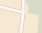
\includegraphics[width=\textwidth]{map.png}}
	%		\fbox{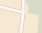
\includegraphics[width=650px]{map.png}}
	\caption{Обзорная карта района работ}
\end{figure}


\section{Гидрогеологические условия площадки и причины подтопления}

Рассматриваемый участок сложен \textit{филлитовыми сланцами, часто встречаются зоны оталькования}. Скальные грунты перекрыты мезозойской корой выветривания, представленной преимущественно суглинками и глинами, образующими водоупорные линзы, на которых формируются временные горизонты приповерхностных подземных вод («верховодка»). Глубина залегания первого устойчивого горизонта подземных вод превышает 15 м.

\textbf{В гидрогеологическом отношении} рассматриваемый участок расположен в пределах Большеуральского сложного бассейна корово - блоковых напорных и безнапорных вод, в области развития палеозойских метаморфических горных пород. С поверхности палеозойские породы на отдельных участках перекрыты спорадически распространенной щебнисто - глинистой корой выветривания и повсеместно - четвертичными отложениями мощностью от первых метров до 5 - 8 м. Подземные воды приурочены к зоне трещиноватости палеозойских интрузивных пород мощностью 40 - 50 м, а в зонах тектонических нарушений и литологических контактов -- до 70 - 80 м. 

Зеркало подземных вод в сглаженном виде повторяет формы рельефа поверхности. Глубина залегания уровня – свыше 15 м. Так как мощность перекрывающих слабо водопроницаемых отложений не выдержана в плане и разрезе, подземные воды недостаточно защищены от поверхностного загрязнения.

По химическому составу подземные воды рассматриваемого района в природных условиях относятся к типу гидрокарбонатных кальциево-магниевых с минерализацией до 0,3 г/дм\textsuperscript{3}, жесткостью 2 - 3 ммоль/дм\textsuperscript{3}. Современное качество воды в условиях интенсивной техногенной нагрузки этой территории претерпело изменения в связи с увеличением в солевом составе воды доли хлоридов и сульфатов. Общая минерализация варьирует в пределах 0,3 - 0,5 г/дм\textsuperscript{3}.

Залегание уровня подземных вод ожидается на глубине свыше 15 м.

В геоморфологическом отношении участок расположен в восточной прибрежной части озера Шарташ. Поверхностный и подземный поток от этого участка направлен в западном направлении в котловину оз. Шарташ.

Осложняющим фактором, вызывающим подтопление на изучаемом участке, является наличие в разрезе водонепроницаемых грунтов, сложная форма кровли суглинков и глин коры выветривания и коренных грунтов, застройка окружающей территории, что вызывает неравномерный напор приповерхностных вод. Источником приповерхностных вод на изучаемом участке являются преимущественно атмосферные осадки и воды, образующиеся в периоды сезонного снеготаяния.

Поскольку устойчивые горизонты подземных вод залегают на глубинах свыше 15\-м, \underline{основной причиной подтопления} является отсутствие сброса собранной ливневыми желобами воды и вследствие этого, накопление ее в приповерхностных грунтах и дальнейшее ее поступление в подвальные помещения.

\begin{figure}[!h]
	\fbox{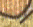
\includegraphics[width=\textwidth]{geomap.png}}
	\caption{Геологическая карта района работ}
\end{figure}


\section{Обоснование выбора типа дренажных \\ мероприятий}

Учитывая гидрогеологические условия площадки и требования к системе дренажа, был выбран вариант вертикального дренажа, представляющего собой  водопоглощающую дренажную скважину глубиной 25 - 30 м.  

Данная скважина работает как дренажно-поглощающий трубчатый колодец - по его стволу приповерхностные воды фильтруются в водопроницаемые трещиноватые грунты, залегающие под  водоупорным горизонтом суглинков (рис. \ref{img:scheme1}). За счет взаимного влияния депрессионных воронок снимаются неравномерности напора приповерхностных вод и локальные области переувлажнения несущих грунтов ликвидируются.

\begin{figure}[!h]
	\centering
	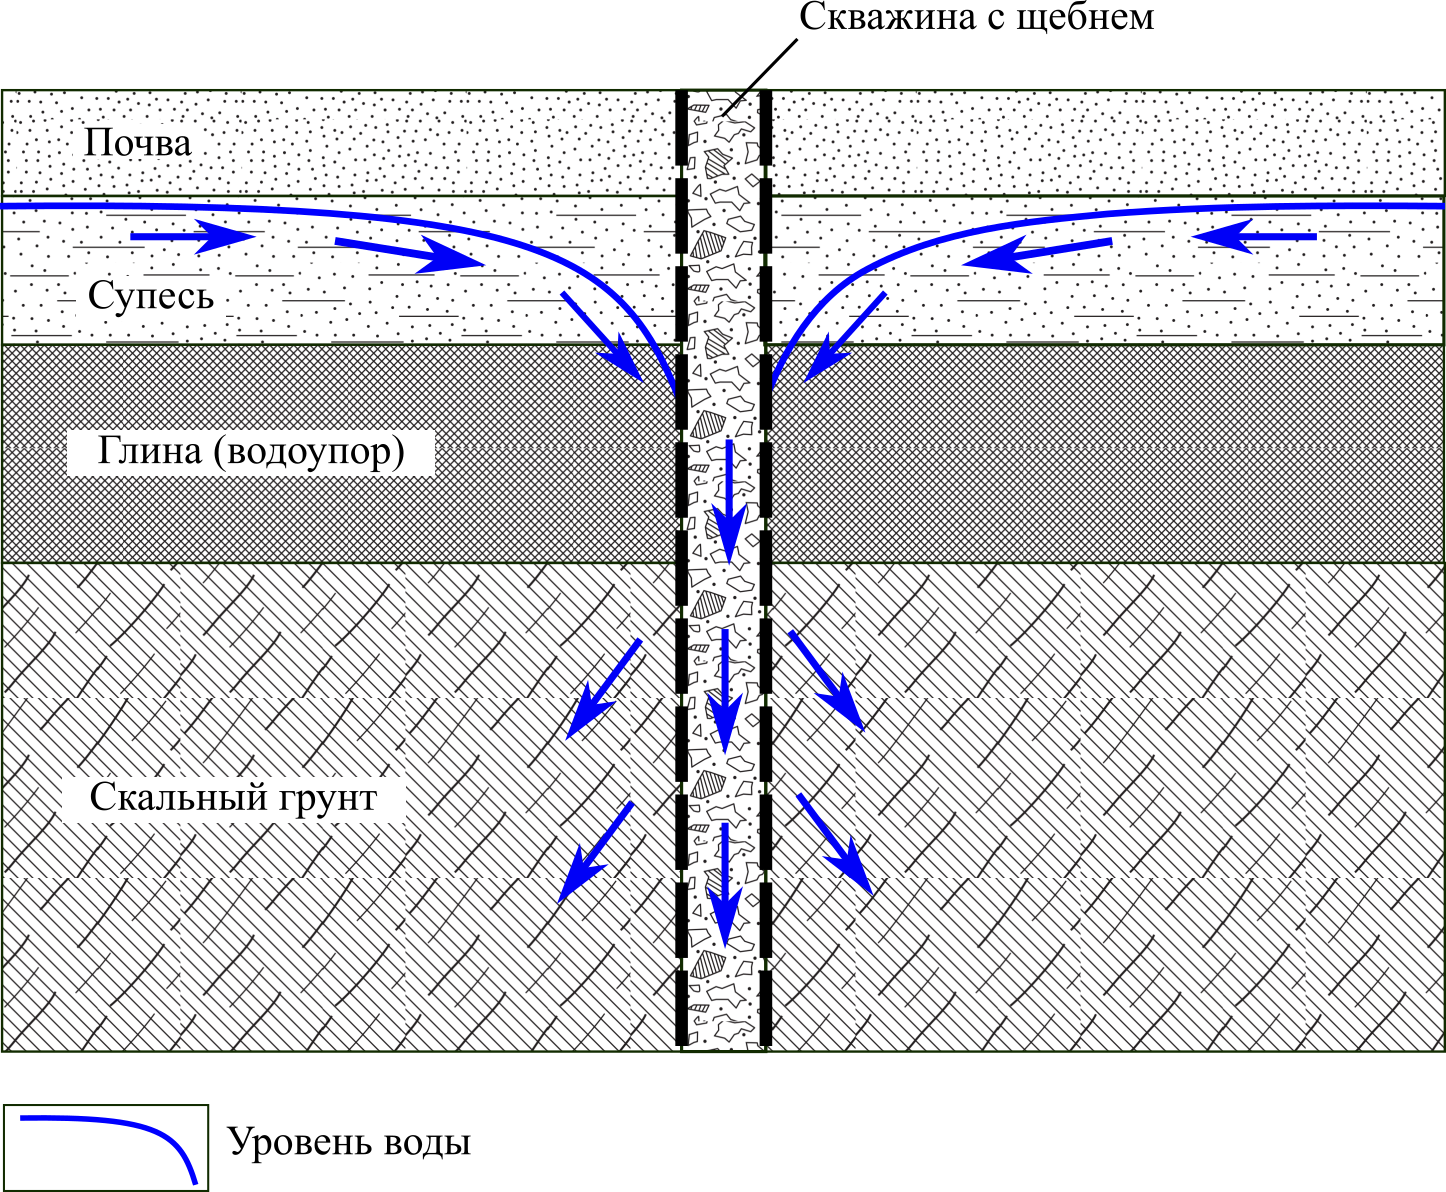
\includegraphics{img1.png}
	\caption[Схема водопонижения]{Схема водопонижения – воды, залегающие на водоупоре, по дренирующей скважине спускаются в трещиноватые скальные грунты}
	\label{img:scheme1}
\end{figure}

Бурение необходимо проводить с обсадными трубами, после проходки скважины на проектную глубину ствол засыпается щебнем, а трубы вынимаются. 
В устье скважины устраивается дренажный колодец, соединяемый с ливневыми желобами. Дренажный колодец засыпается щебнем и закрывается крышкой.

\begin{figure}[!h]
	\centering
%	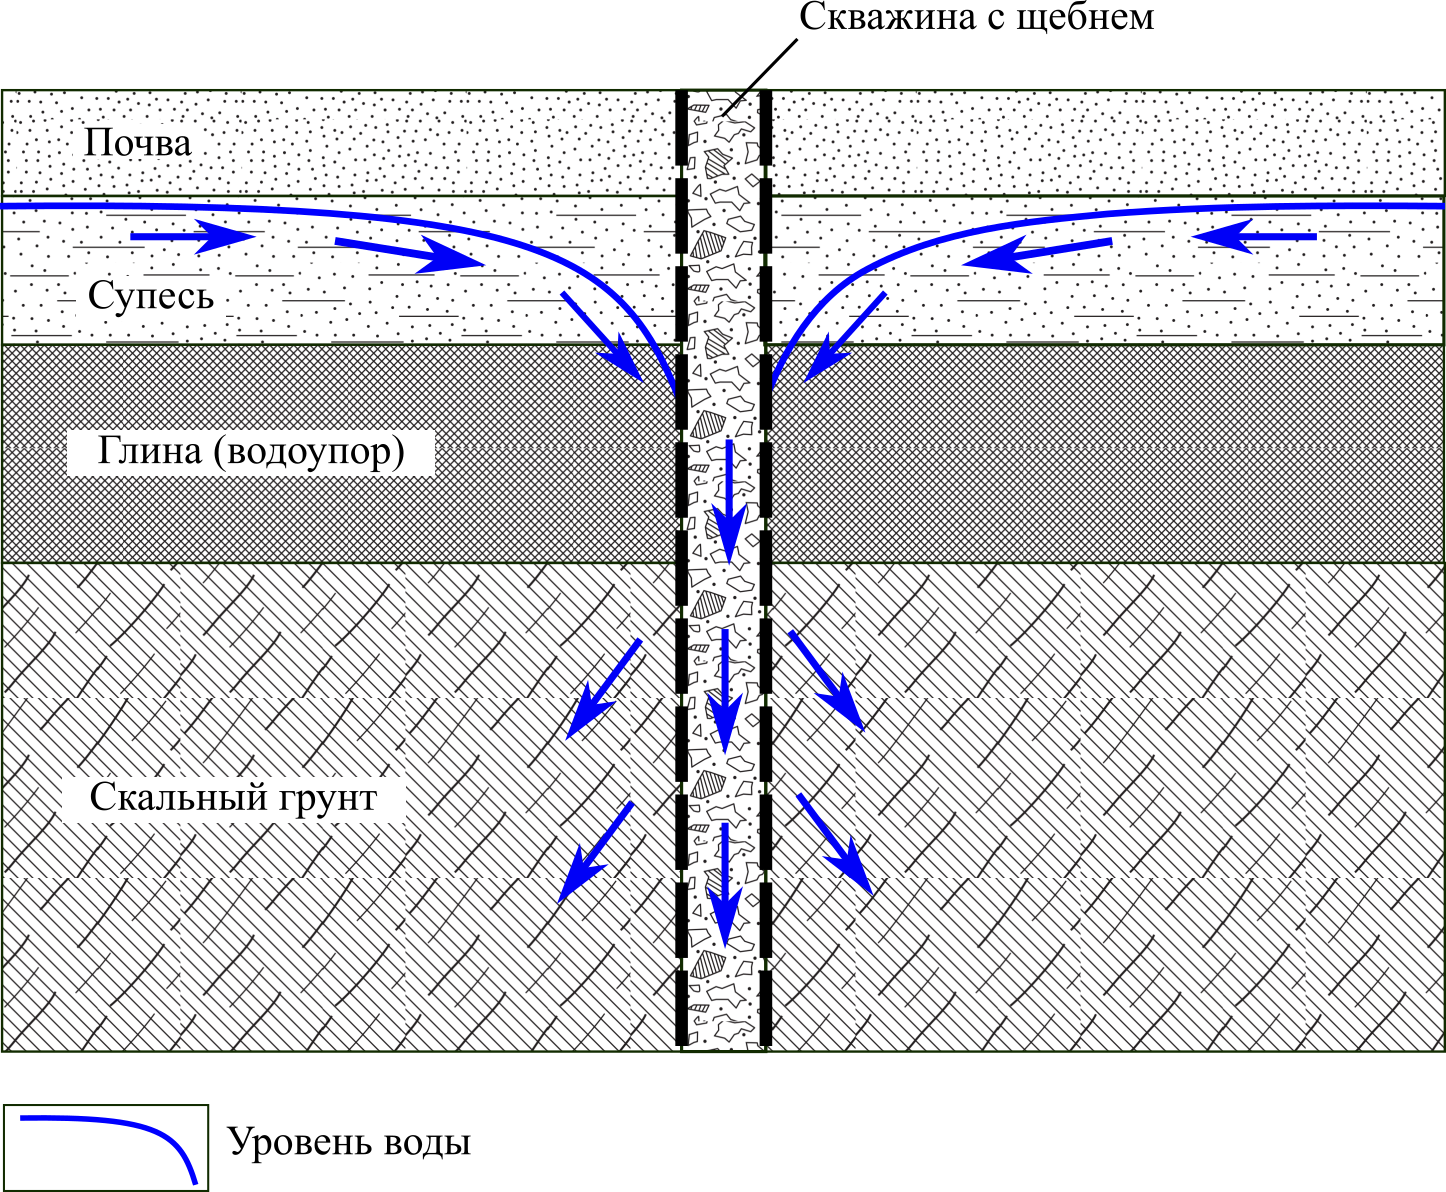
\includegraphics{img1.png}
	\caption{Схема взаимодействия двух скважин}
	\label{img:scheme2}
\end{figure}

По результатам проведенных в сходных геологических условиях в результате пробных откачек отмечается безнапорный характер подземных вод и средний дебит водопоглощающих скважин составляет $1 \, м^3/час$. Коэффициент фильтрации суглинков, залегающих в верхней части разреза, составляет 0,01 м/сут. 

При заложении групповой установки водопонижающих скважин при осушении территории скважины располагают на таком расстоянии, чтобы они влияли друг на друга, то есть расстояние между скважинами должно быть меньше радиуса влияния одиночной скважины. При этом депрессионные воронки от скважин накладываются друг на друга  и уровень воды между скважинами снижается еще больше благодаря интерференции (рис. \ref{img:scheme2}). Чем больше скважин заложено на участке осушения, тем больше снизится уровень воды в произвольно взятой точке, причем общее снижение уровня будет приближенно равно сумме снижений уровня от действия каждой скважины. Наиболее целесообразно располагать скважины на расстоянии  $0,1R$, где $R$ – радиус влияния одиночной скважины в метрах. 

Глубина скважины должна быть достаточной для обеспечения необходимой водозахватной способности выбранной системы дренажа и в то же время она должна быть меньше глубины залегания подземных вод. Исходя из опыта работы авторов настоящего отчета на участках со сходными гидрогеологическими условиями, оптимальной является глубина 25 --- 30 м.


\section{Определение водозахватной способности дрен}

Проверка на достаточность водозахватной способности определяется соблюдением условия:

\begin{equation}\label{eq:debit}
	Q_0 \leqslant f 
\end{equation}

	где 
	
	$Q_0$ -- дебит дрены в $м^3/сут$, 
	
	$f$ -- водозахватная способность

	\bigskip

Расчет водозахватной способности  для вертикальных дрен производится по формуле \mbox{С.К. Абрамова}:

\begin{equation}\label{eq:abramov}
	f = 130 \pi r_c l \sqrt[3]{K}
\end{equation}

	где 

	$f$ -- водозахватная способность дрены в $м^3/сутки$ на одну дрену
	
	$r_c$ -- наружный радиус вертикальных дрен, м
	
	$l$ -- длина фильтра, м
	
	$K$ -- коэффициент фильтрации водоносного пласта в $м^3/сутки$
	
	\bigskip
	
	При $r_c = 0,160 \, м, l = 20 \, м, K = 0,01 \, м^3/сутки $, имеем: $f = 280 \, м^3 / сутки$

	\bigskip
	
При дебите дрены $24 \, м^3/час$ условие \eqref{eq:debit} выполняется. Таким образом, \textbf{водозахватная способность дренажных скважин достаточна} для успешного водопонижения рассматриваемого участка.

\section{Выводы}

\begin{itemize}

\item Изучаемый участок сложен  трещиноватыми  сланцами, перекрытыми слабо водопроницаемыми суглинками и глинами с коэффициентом фильтрации $0,01 \, м^3/сут$. Грунтовые воды, приуроченные к скальным грунтам, залегают на глубинах от 30 м и имеют безнапорный характер.
\item Осложняющим фактором, вызывающим подтопление на изучаемом участке, является наличие в разрезе водонепроницаемых грунтов, сложная форма кровли суглинков и глин коры выветривания и коренных грунтов, застройка окружающей территории, что вызывает неравномерный напор приповерхностных вод.
\item Осложняющим фактором, вызывающим подтопление на изучаемом участке, является наличие в разрезе водонепроницаемых грунтов, сложная форма кровли суглинков и глин коры выветривания и коренных грунтов, застройка окружающей территории, что вызывает неравномерный напор приповерхностных вод.
\item Источником приповерхностных вод на изучаемом участке являются преимущественно атмосферные осадки и воды, образующиеся в периоды сезонного снеготаяния.
\item Поскольку устойчивые горизонты подземных вод залегают на глубинах свыше 15 м, основной причиной подтопления является отсутствие сброса собранной ливневыми желобами воды и вследствие этого, накопление ее в приповерхностных грунтах и дальнейшее ее поступление в подвальные помещения..
\item Приповерхностные воды имеют безнапорный характер.
\item Учитывая гидрогеологические условия площадки и требования к системе дренажа, был выбран вариант вертикального дренажа, представляющего собой водопоглощающую дренажную скважину глубиной 30 м. Данная скважина работает как дренажно-поглощающий трубчатый колодец - по стволам данных скважин приповерхностные воды фильтруются в водопроницаемые трещиноватые грунты, залегающие под  водоупорным горизонтом суглинков (рис. \ref{img:scheme1}). За счет взаимного влияния депрессионных воронок снимаются неравномерности напора приповерхностных вод и локальные области переувлажнения несущих грунтов ликвидируются. 
\item Расчеты показывают, что водозахватная способность примененной системы дренажных скважин достаточна для успешного водопонижения рассматриваемого участка.

\end{itemize}

\section{Технология работ}
\subsection*{Горизонтальный дренаж}
\begin{enumerate}
\item Для сбора дренажных вод на участке по контуру здания проходятся дренажные траншеи на глубину 1,5 - 2,0 м. 
\item В углах поворота траншей устанавливаются дренажные колодцы глубиной 2,0 м диаметром не менее 40 см.
\item На утрамбованное дно траншей насыпают смесь щебня и крупного песка слоем около 10 см, затем укладывают дренажные  трубы (перфорированные полиэтиленовые трубы диаметром 110 мм). Трубы соединяют с отверстиями в дренажном колодце.
\item Дрены засыпаются промытым щебнем или гравием до глубины 50 см от поверхности земли, сверху дрены засыпаются на 20 см песком, а затем вынутым при проходке траншей грунтом. 
\item Чтобы дренажная канава выглядела эстетично, не разрушалась, имелась возможность прохода или проезда, в верхнюю часть канавы желательно установить дренажные лотки ливневой канализации (рис. \ref{img:lotok}) из бетона или пластика (линейные системы водоотвода), соединенные с дренажными колодцами.
\item Дренажные колодцы закрываются крышками.
\end{enumerate}

\begin{figure}[!h]
	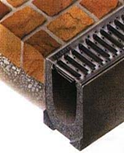
\includegraphics[width=0.2\linewidth]{img2}
	\caption{Дренажный лоток}
	\label{img:lotok}
\end{figure}

\subsection*{Вертикальный дренаж}
\begin{enumerate}
\item Для сброса дренажных вод на участке  бурится дренажная скважина на глубину 30 м с обсадкой перфорированными полиэтиленовыми трубами.
\item В устье дренажной скважины (рис. \ref{img:construction}) производится выемка грунта на ширину дренажного колодца в нижней части  с расширением к верхней части. Ширина выемки в верхней части составляет 2 – 2,5 диаметра дренажного колодца. Глубина выемки 2,5 – 2,7 м. В выемке устанавливается  дренажный колодец. Промежуток между внешними стенками дренажого колодца и стенками выемки засыпается щебнем.
\item Дренажный колодец закрывается крышкой.

\end{enumerate}
\begin{figure}[!h]
	\centering
	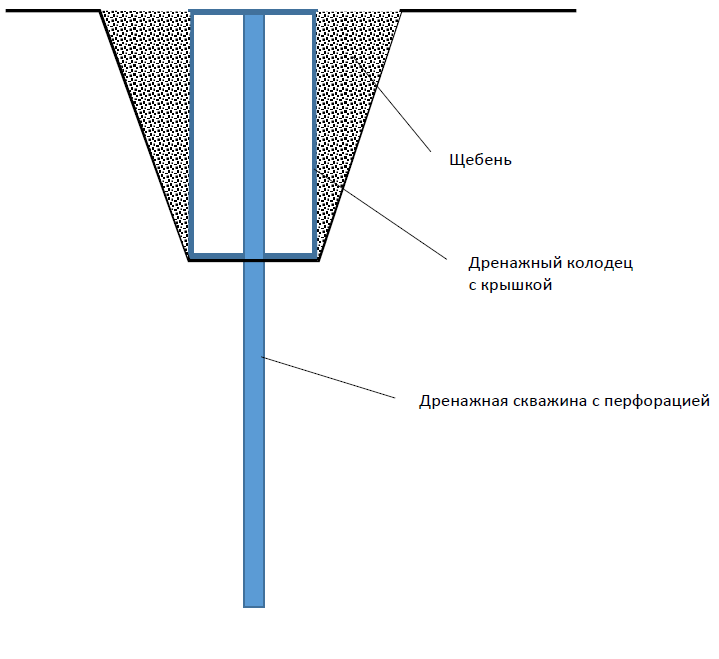
\includegraphics[width=\linewidth]{construction.png}
	\caption[Конструкция]{Конструкция устья дренажной скважины}
	\label{img:construction}
\end{figure}

\begin{figure}[!h]
	\centering
	\includegraphics[height=0.98\textheight]{\txtLegendFname}
	\caption[Условные обозначения]{Условные обозначения к~геологической карте}
	\label{img:legend}
\end{figure}

\end{document} % конец документа

